\documentclass[a4paper,11pt]{article}
\usepackage[utf8]{inputenc}
\usepackage[T1]{fontenc}
\usepackage[french]{babel}
\usepackage{titlesec}
\usepackage{fancyhdr}
\usepackage{geometry}
\usepackage{color}
\usepackage{listings}

\definecolor{light-gray}{gray}{0.95}
\lstset{
backgroundcolor=\color{light-gray},
breaklines=true}

\usepackage{graphicx}
%\usepackage{makeidx}

\usepackage[
breaklinks=true,
colorlinks=true,
linkcolor=black,urlcolor=blue,citecolor=black,
bookmarks=true,bookmarksopenlevel=2]{hyperref}

% Marges %
\geometry{total={210mm,297mm},
left=20mm,right=20mm,
bindingoffset=10mm, 
top=25mm,bottom=25mm}

% Style d'entête %
\pagestyle{fancy}
\lhead{Université de Nantes}
\rhead{2014-2015}
\cfoot{\thepage}

% DOCUMENT %
\widowpenalty=10000 % empeche au maximum la coupure avant la derniere ligne
\clubpenalty=10000  % empeche au maximum la coupure apres la premiere ligne
\raggedbottom       % empeche l'etirement des ressorts verticaux

\begin{document}

\thispagestyle{empty}

{%%%
\sffamily
\centering
\Large
Université de Nantes\\
Faculté des sciences et Techniques\\
Master 1 ALMA\\

~\vspace{\fill}

{\huge 
\textbf{Mini-éditeur de texte}\\Rapport du projet Génie Logiciel
}

\vspace{4cm}

{\LARGE Yvan NOBLET}\\
{\LARGE Julien OUVRARD}\\

\vspace{7cm}

Promoteur :\\ Prof. Gerson Sunyé

\vspace{\fill}

Décembre 2014

%%%
}
\clearpage

%
% ============================================================
% ============================================================
%

\tableofcontents
\clearpage

%
% ============================================================
% ============================================================
%

\section{Présentation du projet mini-éditeur}\label{sec:intro}
\bigskip

C'est dans le cadre de l'UE de Génie Logiciel, que nous avons été amenés à travailler sur le projet d'un mini-éditeur de texte. Le projet portait sur le point de vue structurel du logiciel, c'est pourquoi il ne sera pas question d'interface graphique utilisateur mais de fonctionnalités et de conception.
Ce travail, à réaliser en binôme, nous incite à coder proprement via des schémas reconnus et de comprendre puis tracer le chemin de la spécification à l'implémentation en passant par la conception.
\bigskip

\noindent Le mini-éditeur de texte propose toutes les commandes de base d'un éditeur classique telles que les effets copy, cut, paste, les effets undo/redo et bien évidemment write et backspace. Notre éditeur comporte également la fonctionnalité de créer des macros à partir des commandes citées précédemment.
De plus, une classe utilisateur a été instanciée. Cette dernière permet de simuler l'accès et la modification d'un buffer par plusieurs utilisateurs qui le partage.
\bigskip

\noindent Ainsi, à travers ce rapport nous allons aborder et, si besoin, expliquer le choix des différents logiciels, langages, frameworks et autres patterns utilisés tout au long du projet.

\bigskip
\bigskip
% ===============

\section{Langage \& UML}\label{sec:lang_papy}
\bigskip

\subsection{Scala}\label{subsec:scala}
Le langage utilisé pour réaliser cet éditeur est le \textsc{Scala} dans sa version 2.11.4. Scala est un langage de programmation multi-paradigme, son nom vient de l'anglais \emph{Scalable language} qui peut être traduit par "langage adaptable". Dans notre cas il est utilisé en tant que langage de programmation orienté objet.

\noindent Nous disposons de deux dossiers contenant les sources : src/main et src/test. Dans le premier nous retrouvons le code de chacune des commandes ainsi que celui de l'utilisateur et du buffer, tandis que dans le second se trouve seulement le code concernant les tests.

\subsection{Papyrus}\label{subsec:papyrus}
Afin de modéliser correctement nos classes en UML, nous avons utilsé l'environnement Papyrus intégré à l'IDE Eclipse.
\smallskip

\noindent Papyrus vise à fournir un environnement intégré facile à utiliser pour éditer les modèles de type EMF (Eclipse Modeling Framework), il soutient en particulier UML et les langages de modélisation connexes tels que SysML et MARTE. Papyrus offre également un support très avancé pour les profils UML qui permet aux utilisateurs de définir des éditeurs pour les DSL (Domain Specific Language) basés sur le standard UML 2.

\subsection{Tests}\label{subsec:tests}
Les tests ont été réalisés en suivant le framework JUnit qui prend en charge les tests Scala. Les tests unitaires réalisés portent sur les méthodes des \textbf{Commandes}.

\clearpage

%
% ============================================================
% ============================================================
%

\section{Fonctionnalités de l'éditeur}\label{sec:fonc}
\bigskip

\subsection{Le Buffer}\label{subsec:buffer}
\bigskip

\large{\textbf{Buffer}}
\medskip

\noindent Le \emph{Buffer} représente le c\oe{}ur de l'éditeur. C'est l'espace de travail avec lequel les différentes commandes vont interagir.
Le buffer est constitué d'un \textit{contenu} et d'un \textit{index} et des objets \textbf{Clipboard}, \textbf{Selectionner} et \textbf{Historique} qui seront détaillés par la suite.
\smallskip

\noindent Le \textit{contenu} est de type \textbf{String} et représente ce qui est écrit dans par les utilisateurs dans le mini-éditeur de texte.
\smallskip

\noindent L'\textit{index} est de type \textbf{int} et nous sert à nous repérer dans l'historique. \'A chaque modification du \textit{contenu} l'index est incrémenté.

\bigskip

\large{\textbf{Clipboard}}
\medskip

\noindent Le \emph{Clipboard} représente le presse-papier d'un buffer. C'est ici que sera enregistrée une sélection copiée ou coupée. Le presse-papier reste le même du moment qu'il n'y a pas de nouvelle sélection (copiée ou coupée) qui l'écrase.
\smallskip

\noindent Le presse-papier est simplement constitué d'un \textit{contenu} de type \textbf{String} qui est une sous-chaîne du contenu du buffer.
\bigskip

\large{\textbf{Selectionner}}
\medskip

\noindent L'objet \emph{Selectionner} permet la sélection d'une sous-chaîne du contenu du buffer. Plus précisément, dans le projet c'est un objet constitué de deux index représentant un intervalle et d'une chaîne de caractère représentant la sélection. Si l'intervalle est nul, il s'agit d'un curseur et la chaîne est vide.
\bigskip

\large{\textbf{Historique}}
\medskip

\noindent L'\emph{Historique} représente la mémoire du buffer. Il contient toutes les modifications auxquelles le buffer a été sujet. Il permet, grâce aux commandes \textbf{Annuler} et \textbf{Refaire} (que nous verrons ensuite), de revenir à un état antérieur du buffer via un \textbf{Memento}.
\bigskip

\large{\textbf{Memento}}
\medskip

\noindent Le \emph{Memento} est l'état d'un buffer entre deux modifications. Il mémorise le contenu (\textbf{String}) du buffer ainsi que la position (\textbf{int}) de son curseur à cet instant.
\bigskip

\subsection{L'Utilisateur}\label{subsec:user}
\bigskip

\large{\textbf{Utilisateur}}
\medskip

\noindent L'\emph{Utilisateur} est un \textbf{Observateur}, c'est-à-dire qu'il est abonné à un ou plusieurs \textbf{Buffer} et qu'il sera notifié dès que ceux-ci seront modifiés par un autre utilisateur.
\smallskip

\noindent Un utilisateur possède simplement un \textit{nom} de type \textbf{String}.
\bigskip

\large{\textbf{Observateur}}
\medskip

\noindent L'\emph{Observateur} est une classe abstraite. Un observateur est notifié par l'objet observable auquel il est abonné lorsque ce dernier le souhaite.
\bigskip

\large{\textbf{Observable}}
\medskip

\noindent L'\emph{Observable} est une classe abstraite. Un observable contient une liste d'\textbf{Observateurs} qui y sont abonnés.
\bigskip

\subsection{Les commandes}\label{subsec:commandes}
\bigskip

\large{\textbf{Commande}}
\medskip

\noindent La classe abstraite \emph{Commande} permet une généricité des exécutions des commandes qui suivent, en particulier lors de l'utilisation de \textbf{Macros}.
\bigskip

\large{\textbf{Ecrire}}
\medskip

\noindent L'objet \emph{Ecrire} permet simplement d'ajouter du contenu de type \textbf{String} dans le buffer suivant la position du curseur.
\bigskip

\large{\textbf{Effacer}}
\medskip

\noindent L'objet \emph{Effacer} efface soit un caractère du contenu du buffer, soit une sélection si une sélection a été faite au préalable.
\bigskip

\large{\textbf{Copier}}
\medskip

\noindent L'objet \emph{Copier} sauvegarde la sélection (de type \textbf{String}) dans le \textbf{Clipboard}.
\bigskip

\large{\textbf{Couper}}
\medskip

\noindent Comme l'objet \textbf{Copier}, \emph{Couper} sauvegarde la sélection dans le \textbf{Clipboard}, en revanche il effectue aussi une suppression de la sélection dans le contenu du buffer.
\bigskip

\large{\textbf{Coller}}
\medskip

\noindent \emph{Coller} permet d'ajouter le contenu du \textbf{Clipboard} au contenu du \textbf{Buffer} selon la position du curseur ou à la place d'une sélection.
\bigskip

\large{\textbf{Annuler}}
\medskip

\noindent La commande \emph{Annuler} propose la possibilité à l'utilisateur de revenir en arrière dans ses modifications du buffer. Grâce à l'\textbf{Historique} le buffer peut reprendre un état passé.
\bigskip

\large{\textbf{Refaire}}
\medskip

\noindent La commande \emph{Refaire} permet le déplacement inverse de la commande \textbf{Annuler} et ainsi revenir à l'état présent du buffer, toujours grâce à l'\textbf{Historique}.
\bigskip

\large{\textbf{Macro}}
\medskip

\noindent Finalement la \emph{Macro} offre la possibilité à l'utilisateur de combiner plusieurs des commandes vues précédemment en une seule nouvelle commande.
\smallskip

\noindent Cet objet contient une liste de \textbf{Commande} qui s'exécuteront les unes à la suite des autres en un seul appel selon la configuration choisie.
\bigskip

\clearpage

%
% ============================================================
% ============================================================
%

\section{Patrons de conceptions}\label{sec:pattern}
\bigskip

\subsection{Memento}\label{subsec:memento}
Le patron de conception Memento nous a été utile pour implémenter les commandes \textbf{Annuler}(undo) et \textbf{Refaire}(redo). Il se compose des classes \textbf{Historique}, \textbf{Memento} et \textbf{Buffer}.
La classe \emph{Memento} sauvegarde l'état du \emph{Buffer} et la position du curseur. La classe \emph{Historique}, quant à elle, sauvegarde une liste de Memento et permet ainsi d'aller et venir dans les différents états sauvegardés. Enfin, la classe \emph{Buffer}, qui représente l'espace de travail, est la classe dont on enregistre l'état courant à chaque modification (toute modification affectant son contenu).
Le pattern permet initialement de récupérer n'importe quel état par son index. Dans ce projet il est utilisé de manière bien spécifique puisqu'on ne se déplace que par états suivants ou précédents pour respecter les fonctionnalités des commandes \emph{Annuler} et \emph{Refaire}.
\smallskip

\noindent Une fois implémentées, les commandes permettent d'annuler ou de refaire une(des) opération(s) à volonté.

\vspace{2cm}

\begin{figure}[h!]
   \centerline{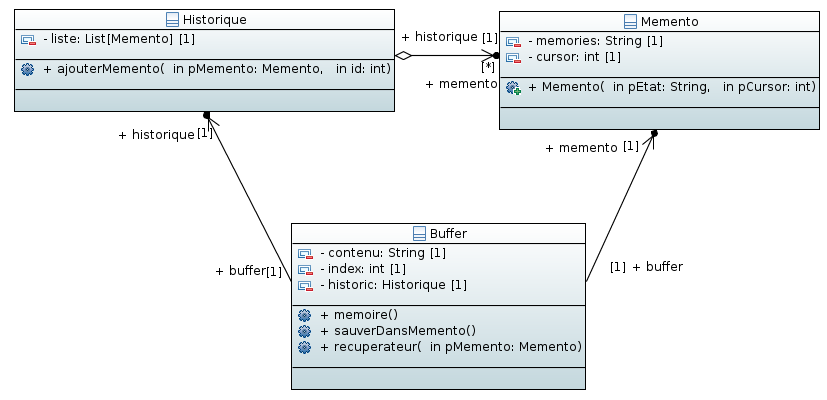
\includegraphics[scale=0.7]{DiagrammeMemento.png}}
   \caption{\label{diaMemento} Diagramme UML du patron de conception \emph{Memento}}
\end{figure}

\vspace{2cm}

\noindent Malgré un ajustement énoncé plus haut, l'utilisation et l'implémentation de ce patron de conception fut assez évidente avec le principe d'historique. Il garde en effet tout en mémoire, ce qui est ce que nous recherchons lorsque nous souhaitons pouvoir nous déplacer à travers les différents états qu'a pu avoir un objet.

\clearpage

%
% ============================================================
% ============================================================
%

\subsection{Observer}\label{subsec:observer}
Le patron Observer permet à plusieurs \textbf{Utilisateurs} abonnés à un même \textbf{Buffer} d'être notifiés à chaque mise à jour du contenu du buffer, de ce fait lorsqu'un utilisateur écrira dans un buffer, tous les utilisateurs abonnés à ce buffer le verront. De plus un \emph{Utilisateur} peut être abonné à plusieurs \emph{Buffer}.
\smallskip

\noindent Ce pattern est composé des classes \textbf{Observable}, \textbf{Observateur}, \textbf{Utilisateur} et \textbf{Buffer}.

\vspace{2cm}

\begin{figure}[h!]
   \centerline{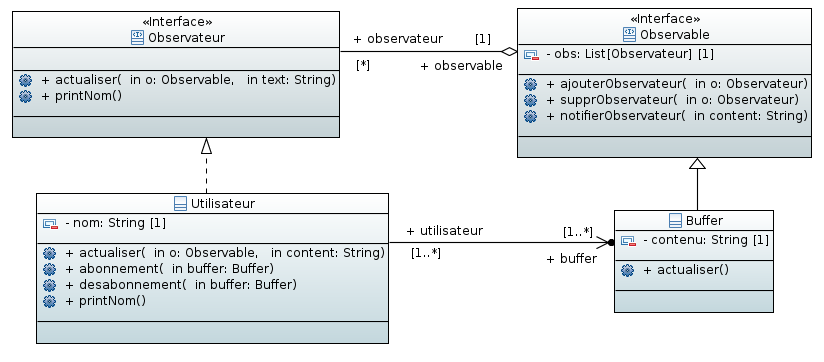
\includegraphics[scale=0.7]{DiagrammeObserver.png}}
   \caption{\label{diaObserver} Diagramme UML du patron de conception \emph{Observer}}
\end{figure}

\vspace{2cm}

\noindent Le patron de conception Observer permet ici de simuler un partage des données entre plusieurs utilisateurs. Un partage synchronisé en ligne d'un éditeur de texte serait un peu plus complexe mais l'idée reste la même.
\clearpage

%
% ============================================================
% ============================================================
%

\subsection{Command \& Composite}\label{subsec:com&com}
Toutes les commandes exécutables par les utilisateurs sur notre éditeur ont été implémentées en respectant le patron de conception Command. La possibilité de réaliser des macros quant à elle suit le schéma du patron Composite. Ces deux patterns fonctionnent en paire dans l'éditeur puisqu'il nous fallait une méthode commune et générique à toutes les commandes pour la création de macro qui est une composition de commandes.
\smallskip

\noindent Ces patterns sont représentés par les classes \textbf{Commande}, \textbf{Macro}, \textbf{Buffer}, et toutes les classes de \textbf{Commandes} basiques de l'éditeur.

\vspace{2cm}
\large{\textbf{Command}}

\begin{figure}[h!]
   \centerline{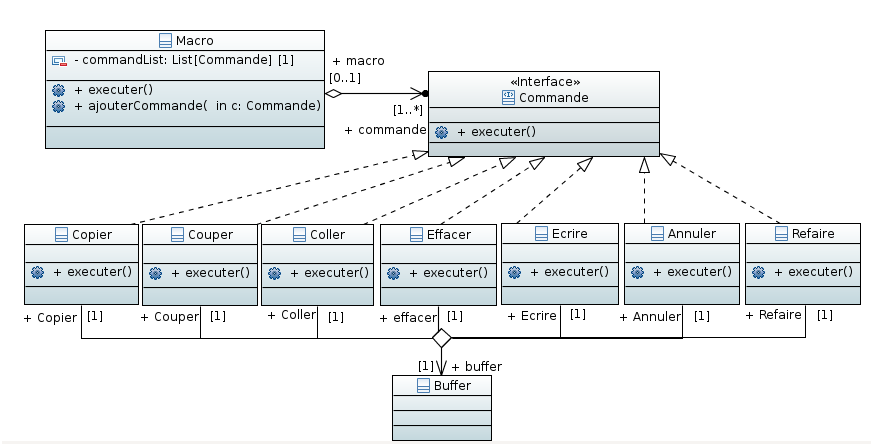
\includegraphics[scale=0.7]{DiagrammeCommand.png}}
   \caption{\label{diaCommand} Diagramme UML du patron de conception \emph{Command}}
\end{figure}

\vspace{2cm}
\noindent Dans notre projet il existe en réalité deux invocateurs des commandes à savoir \textbf{Macro} et \textbf{Buffer}. Ce dernier se trouve être également le récepteur.
\smallskip

\noindent L'invocateur ne connaît pas le l'intérieur des \textbf{Commandes} il leur demande juste de s'exécuter. Il ne connaît pas non plus le récepteur, nous préservons ainsi l'encapsulation.

\clearpage

%
% ============================================================
% ============================================================
%

\large{\textbf{Composite}}

\begin{figure}[h!]
   \centerline{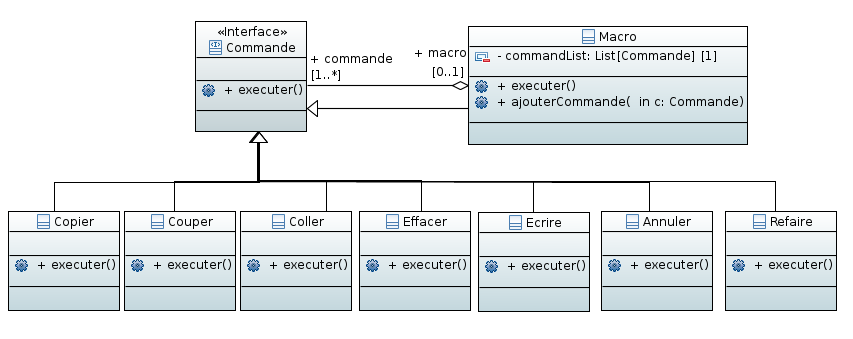
\includegraphics[scale=0.7]{DiagrammeComposite.png}}
   \caption{\label{diaComposite} Diagramme UML du patron de conception \emph{Composite}}
\end{figure}

\vspace{2cm}
\noindent Toutes les commandes de base de l'éditeur interagissent avec le buffer via une seule méthode générique : \textit{executer()}. En plus de simplifier la compréhension du code et de le rendre plus maintenable, l'implémentation de ce pattern permet la création de macros beaucoup plus facilement. Grâce à cette méthode générique toutes les commandes seront appelées de la même façon.

\clearpage

%
% ============================================================
% ============================================================
%

\section{Conclusion}\label{sec:conclusion}
\bigskip

Ce projet nous a permis de nous remémorer les design patterns vus en licence 3, de nous familiariser avec le langage objet Scala et les tests JUnit et d'apprendre à perdre moins de temps sur Papyrus et Maven.
\bigskip

\noindent En effet, l'année dernière en troisième année de licence informatique nous avons vu les design patterns lors du module de Programmation Orienté Objet, c'est avec joie que nous les avons retrouvés tout au long de ce projet. L'idée de patron de conception est assez intéressante, ils permettent souvent une simplification et une compréhension universelle du code. Ils sont, en revanche, pour nous encore assez difficile à penser au sein d'un code. Nous ne pensons pas automatiquement à l'implémentation d'un pattern en voyant tels ou tels types de méthodes. Ce projet nous aura aidés à y voir encore un peu plus clair dans ce domaine.
\bigskip

\noindent Scala et les JUnit tests sont tout nouveaux pour nous. Nous n'avions jamais eu à nous en servir dans notre jeune passé de développeurs. Scala étant proche du Java fut globalement assez simple à prendre en main, nous n'avons pas eu de difficulté particulière ni de blocage sévère. De même que pour Scala, JUnit dans l'utilisation que nous en avons faite fut facile d'approche.
\bigskip

\noindent Là où nous avons en revanche perdu énormément de temps au cours du projet furent les parties en relation avec Papyrus et Maven. Nous n'avions jamais eu à utiliser ces frameworks et nous ne les avons pas trouvé très intuitifs. Nous avons essayé de faire de notre mieux selon ce que nous avons compris.
\bigskip

Ce fut dans l'ensemble un projet vraiment intéressant nous initiant à de nouveaux frameworks et proposant un la conception et l'implémentation d'un logiciel sous un nouvel angle, plus professionel que ce que nous avons fait jusque-là.

\bigskip
\bigskip
% ===============

\clearpage

%
% ============================================================
% ============================================================
%

\section{Annexe}\label{sec:annexe}
\bigskip

\begin{figure}[h!]
   \centerline{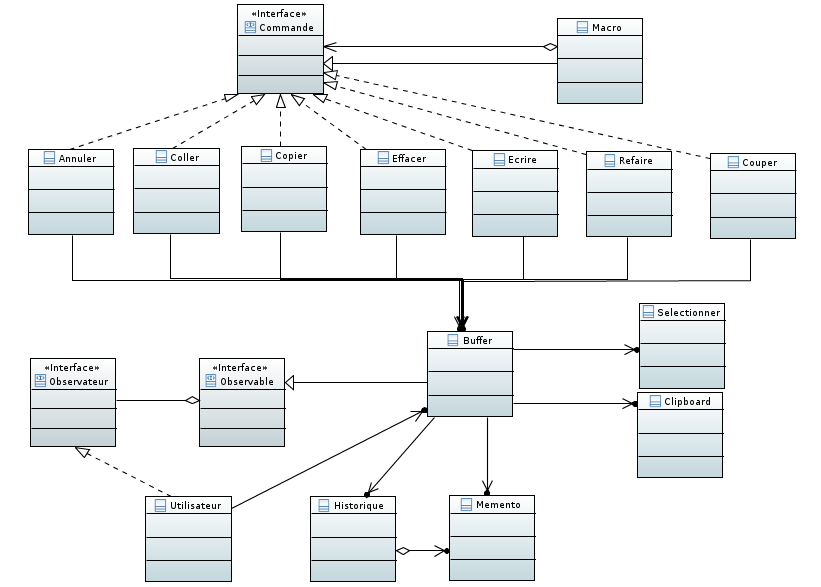
\includegraphics[angle=90, scale=1]{DiagrammeGlobal.png}}
   \caption{\label{diaEditeur} Diagramme UML du mini-éditeur}
\end{figure}

\clearpage

%
% ============================================================
% ============================================================
%

\end{document}